% --------------------------------------------------------------------------------------------------
% Section: Prognostic Indicators
% This section covers key factors that affect prognosis in lung cancer,
% including survival rates, recent trends, and clinical determinants.
% --------------------------------------------------------------------------------------------------

\section{Prognostic Indicators}

% --------------------------------------------------------------------------------------------------
% Subsection: Survival Rates and Trends
% Introduces the importance of survival rates in lung cancer,
% highlights differences by cancer type and stage,
% and discusses recent improvements due to screening and therapies.
% --------------------------------------------------------------------------------------------------

\subsection{Survival Rates and Trends}

% Overview of survival rates as measures of disease impact and treatment success.
Survival rates in lung cancer are important indicators of disease burden, therapeutic success, and 
early detection effectiveness. These rates vary significantly depending on cancer type, stage at 
diagnosis, patient demographics, and treatment accessibility.

% Explanation of survival differences between major lung cancer types.
Non-small cell lung cancer (NSCLC), which comprises around 85\% of lung cancer cases, typically has 
a better prognosis than small cell lung cancer (SCLC), which is more aggressive and fast-growing. 

% Presentation of key survival statistics with citation.
According to global cancer statistics, the 5-year survival rate for localized NSCLC is approximately 
64\%, but this rate drastically drops to 8\% for distant-stage disease \cite{cancerstats2023}.

% Recent advances improving survival: early detection, targeted and immune therapies.
In recent years, survival trends have improved slightly due to advances in early detection through 
low-dose CT screening, the development of targeted therapies, and immunotherapies. Studies have 
shown that overall mortality from lung cancer has declined in high-income countries, particularly in 
populations with reduced smoking rates and improved healthcare access \cite{siegeletc2022trends}.

% Visual representation of survival trends over time.
\vspace{1em}
\begin{center}
    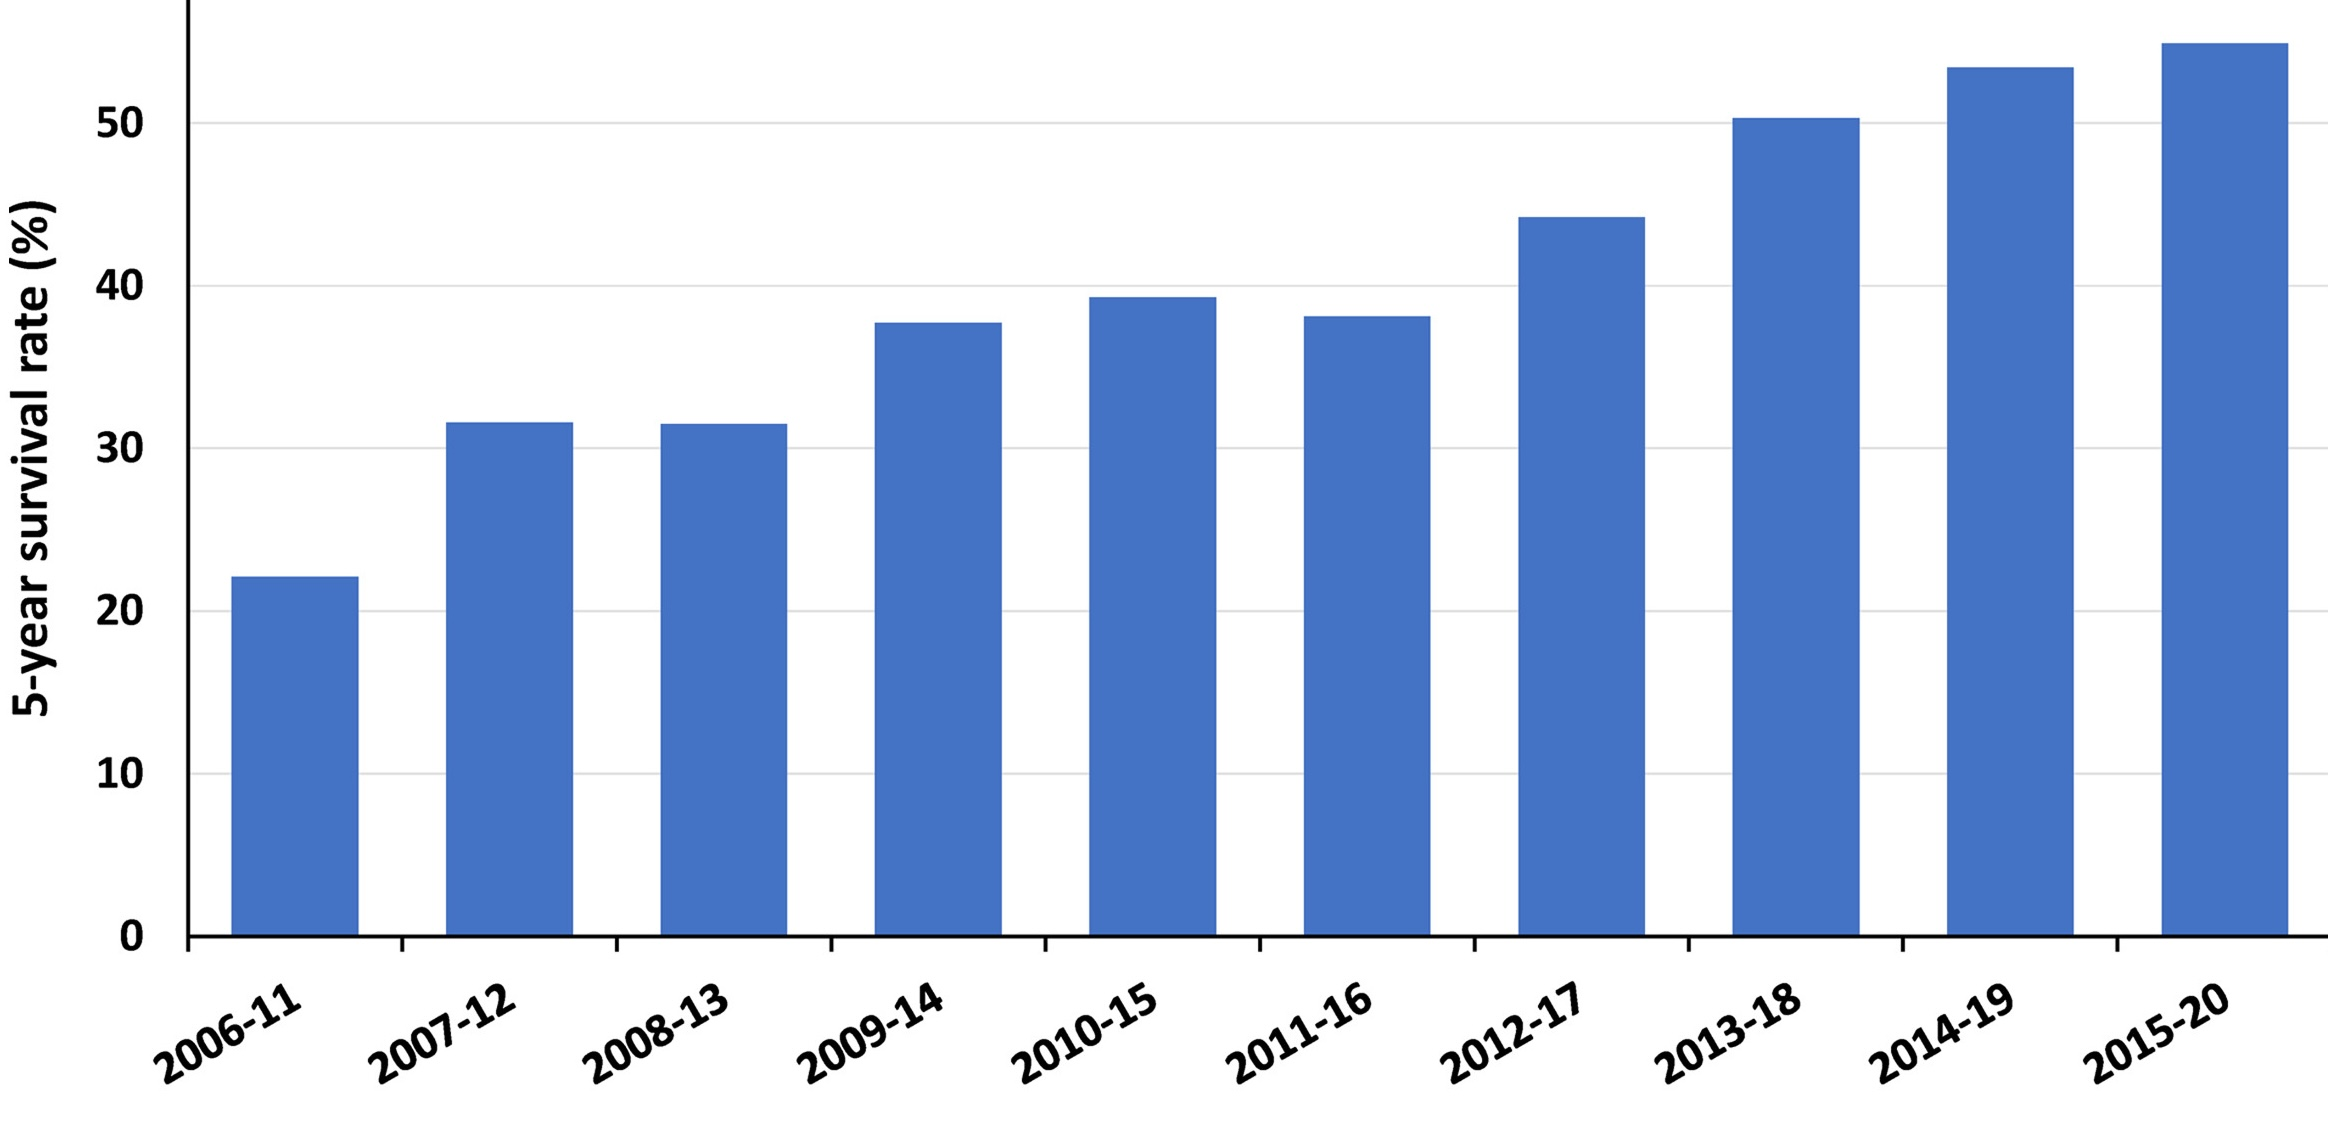
\includegraphics[width=1.00\textwidth]{../assets/05-prognosis/survival-rates.jpg}

    % Caption with source citation for the figure.
    \small\textit{Five-year survival rates over years (all stages). \cite{osarogiagbon2023stage}}
\end{center}
\vspace{1em}

% Despite improvements, lung cancer remains highly lethal globally.
However, despite these improvements, lung cancer remains one of the leading causes of cancer-related 
deaths worldwide. The global 5-year survival rate for all lung cancers combined remains below 20\%, 
underlining the need for continued progress in early detection and treatment strategies 
\cite{bray2018global}.

% --------------------------------------------------------------------------------------------------
% Subsection: Determinants of Clinical Outcome
% Discusses key clinical and biological factors influencing prognosis,
% with detailed points on stage, histology, performance, genetics, comorbidities, and smoking.
% --------------------------------------------------------------------------------------------------

\subsection{Determinants of Clinical Outcome}

% Introduction to clinical, biological, and lifestyle factors affecting prognosis.
Several clinical, biological, and lifestyle factors influence the prognosis of lung cancer patients. 
These determinants help clinicians estimate disease progression and tailor personalized treatment 
strategies.

\begin{itemize}
    % Stage at diagnosis as the most critical prognostic factor.
    \item \textbf{Stage at Diagnosis:} The single most important prognostic factor. Patients 
    diagnosed at early stages (I or II) typically have much better outcomes than those diagnosed at 
    advanced stages (III or IV). Early-stage lung cancer is often amenable to surgical resection or 
    curative radiotherapy, which significantly improves survival chances \cite{goldstaging}.
\end{itemize}

% Figure showing survival rates by stage over time in a specific hospital.
\vspace{1em}
\begin{center}
    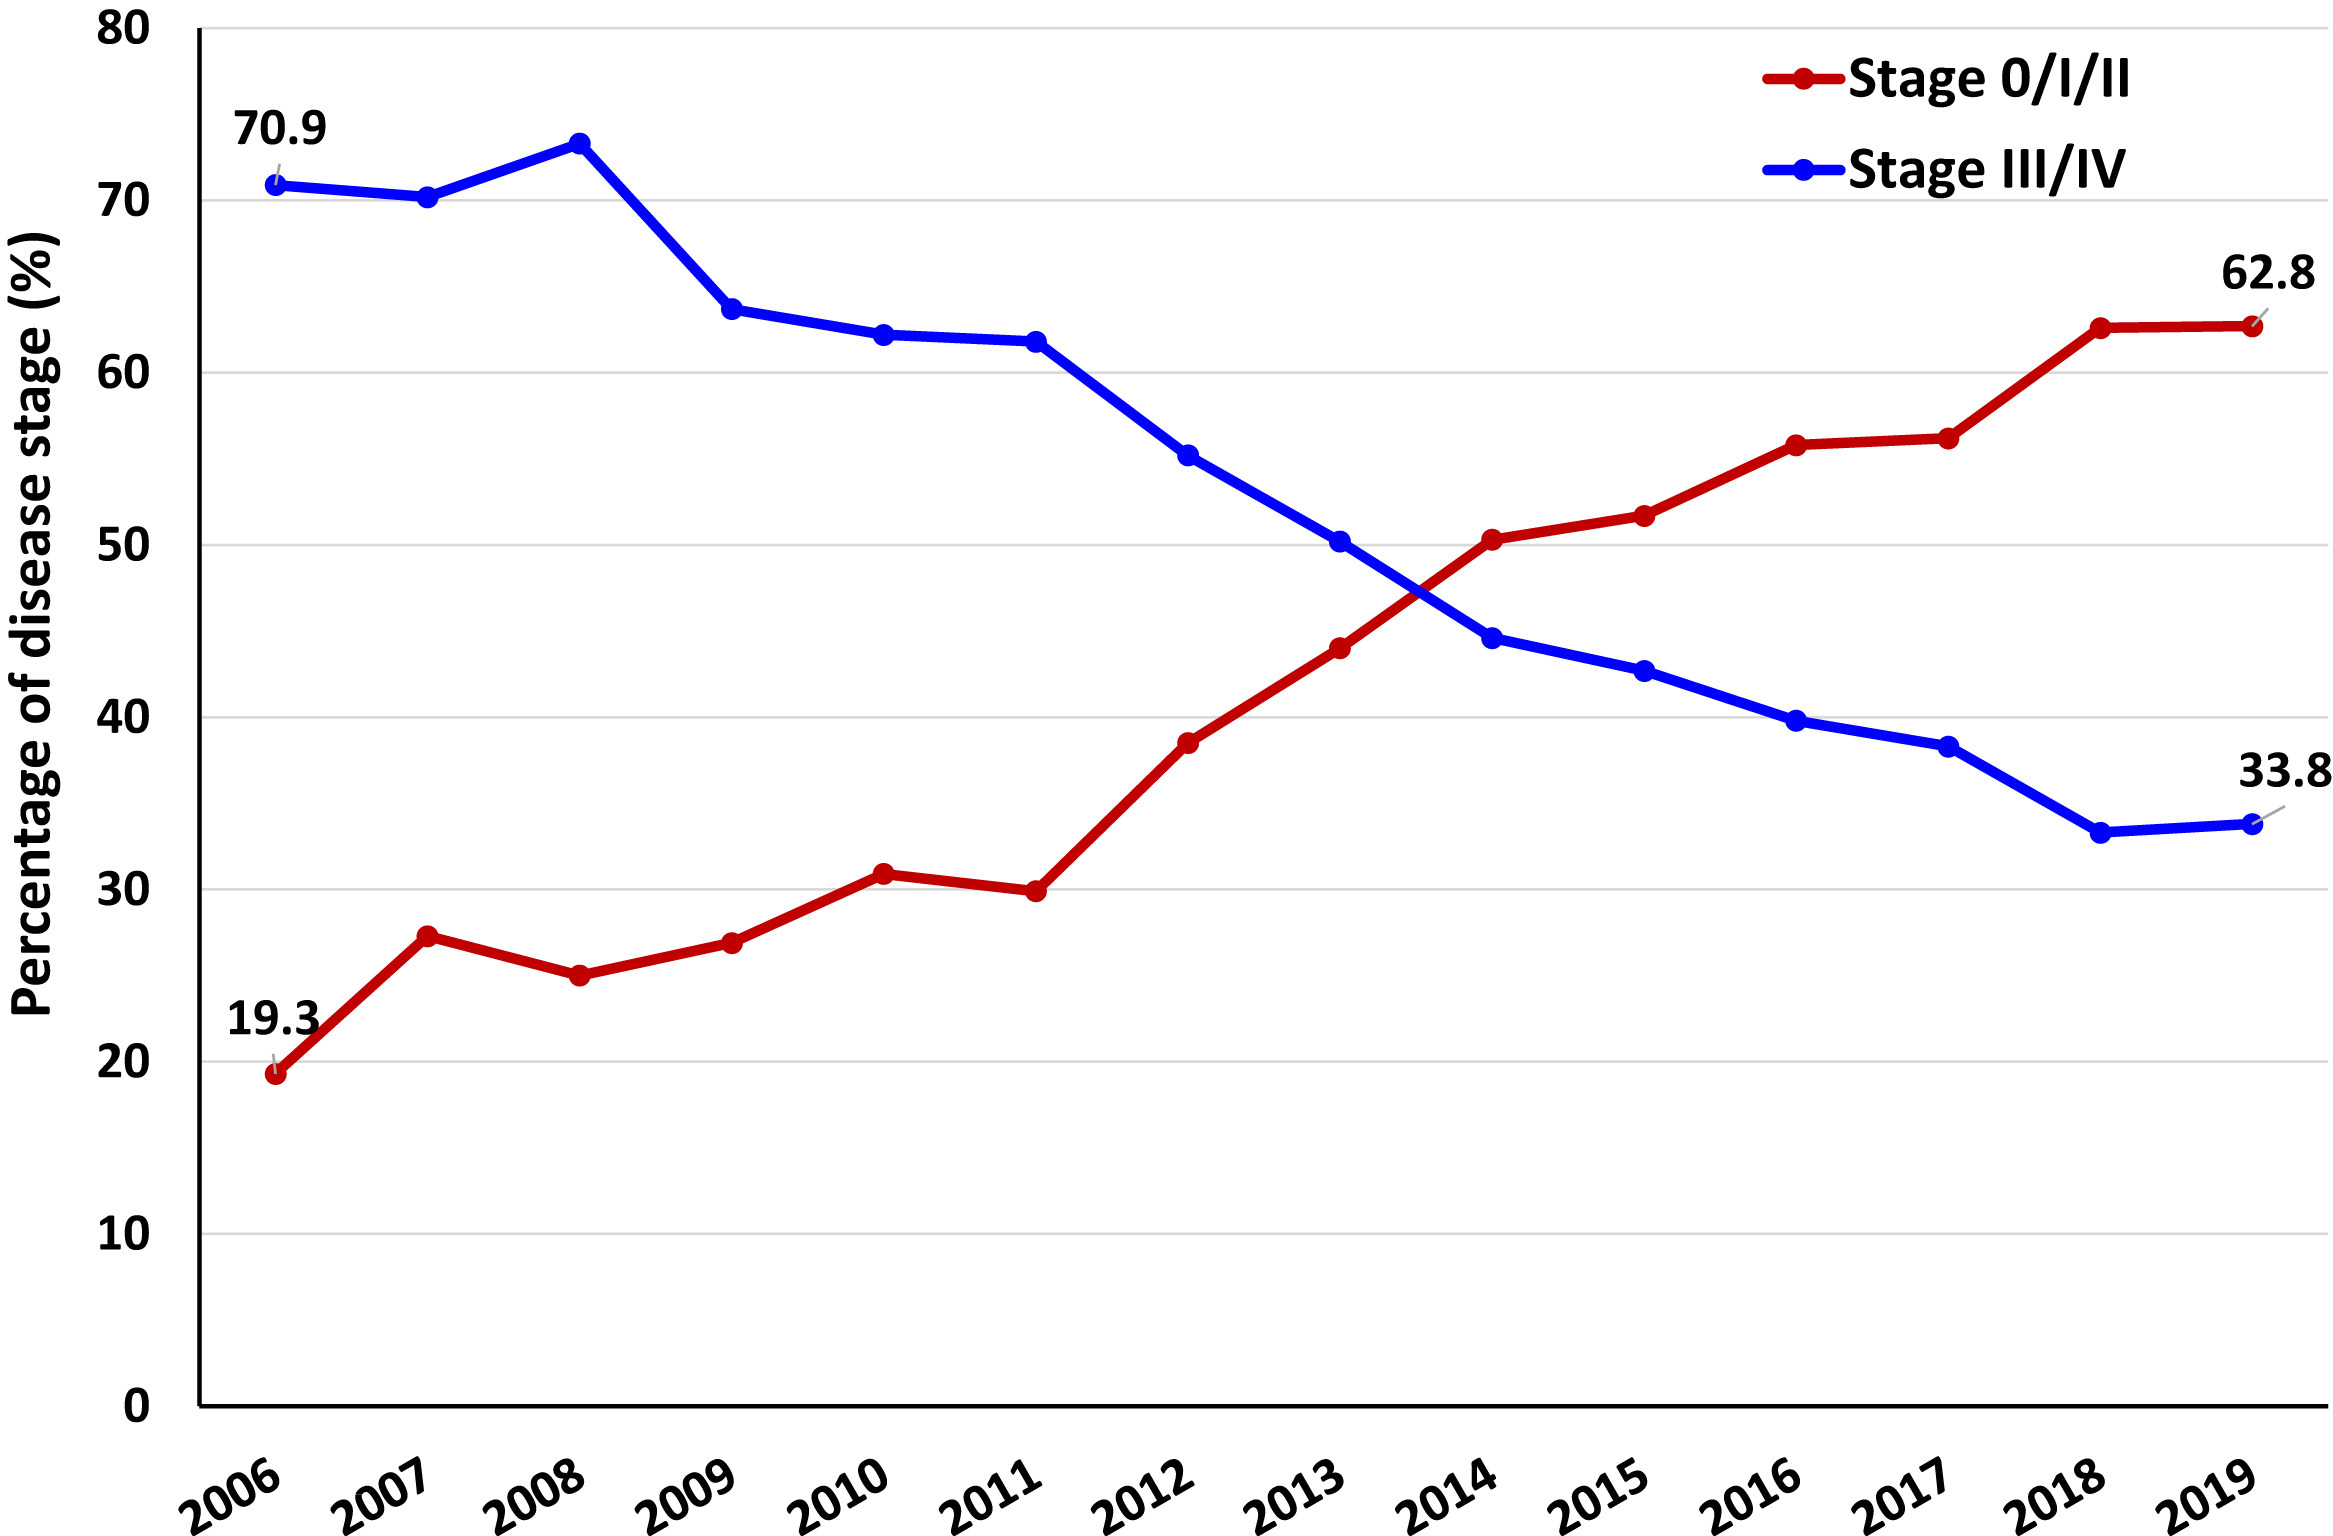
\includegraphics[width=1.00\textwidth]{../assets/05-prognosis/stage-survival-rates.jpg}

    % Caption includes abbreviation explanation and source.
    \small\textit{Change in localized (stage 0/I/II) and advanced (stage III/IV) lung cancer from 
    2006 to 2019 in NTUH. NTUH, National Taiwan University Hospital. \cite{osarogiagbon2023stage}}
\end{center}
\vspace{1em}

\begin{itemize}
    % Histological subtype impacts prognosis.
    \item \textbf{Histological Type:} The type of lung cancer, such as adenocarcinoma, squamous cell 
    carcinoma, or small cell carcinoma, impacts prognosis. For example, adenocarcinomas are 
    generally associated with better outcomes, while SCLC tends to have a more rapid progression and 
    worse prognosis \cite{travis2015classification}.
\end{itemize}

% Survival curves comparing NSCLC and SCLC patients, resected and unresected.
\vspace{1em}
\begin{center}
    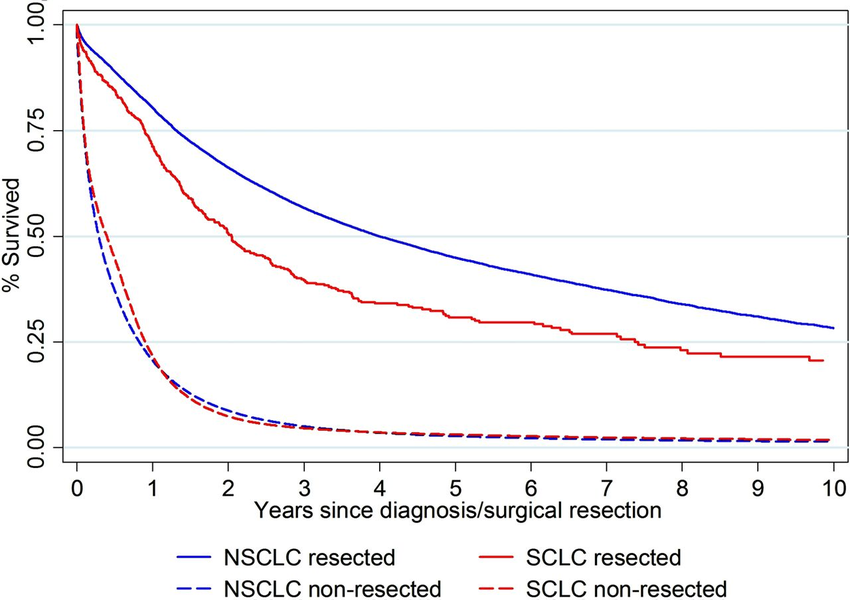
\includegraphics[width=1.00\textwidth]{../assets/05-prognosis/histological-type-survival.png}

    \small\textit{Kaplan–Meier survival analysis of resected and unresected patients with non-small 
    cell lung cancer (NSCLC) and small cell lung cancer (SCLC). \cite{article}}
\end{center}
\vspace{1em}

\begin{itemize}
    % Performance status describes patient's overall health and treatment tolerance.
    \item \textbf{Performance Status:} A measure of a patient’s general well-being and ability to 
    perform daily activities. Patients with good performance status tend to tolerate aggressive 
    treatments better and have improved survival outcomes \cite{basch2016symptoms}.

    % Genetic markers guide prognosis and targeted therapies.
    \item \textbf{Genetic and Molecular Markers:} Certain genetic mutations, such as EGFR, ALK, or 
    KRAS, can influence prognosis and guide the use of targeted therapies. For example, patients 
    with EGFR mutations may benefit significantly from tyrosine kinase inhibitors, improving 
    survival outcomes \cite{molecular2023}.

    % Presence of comorbidities affects treatment and outcomes.
    \item \textbf{Comorbidities:} The presence of other chronic conditions such as chronic 
    obstructive pulmonary disease (COPD), cardiovascular disease, or diabetes can affect treatment 
    options and survival \cite{copdlungcancer}.
\end{itemize}

\begin{itemize}
    % Smoking status as a modifiable risk factor influencing prognosis.
    \item \textbf{Smoking Status:} Non-smokers or those who have quit smoking tend to have better 
    clinical outcomes compared to current smokers. Continued tobacco exposure during treatment can 
    reduce the efficacy of therapies and worsen prognosis \cite{gilbert2020smoking}.
\end{itemize}

% Figure showing impact of smoking reduction on lung cancer risk in COPD patients.
\vspace{1em}
\begin{center}
    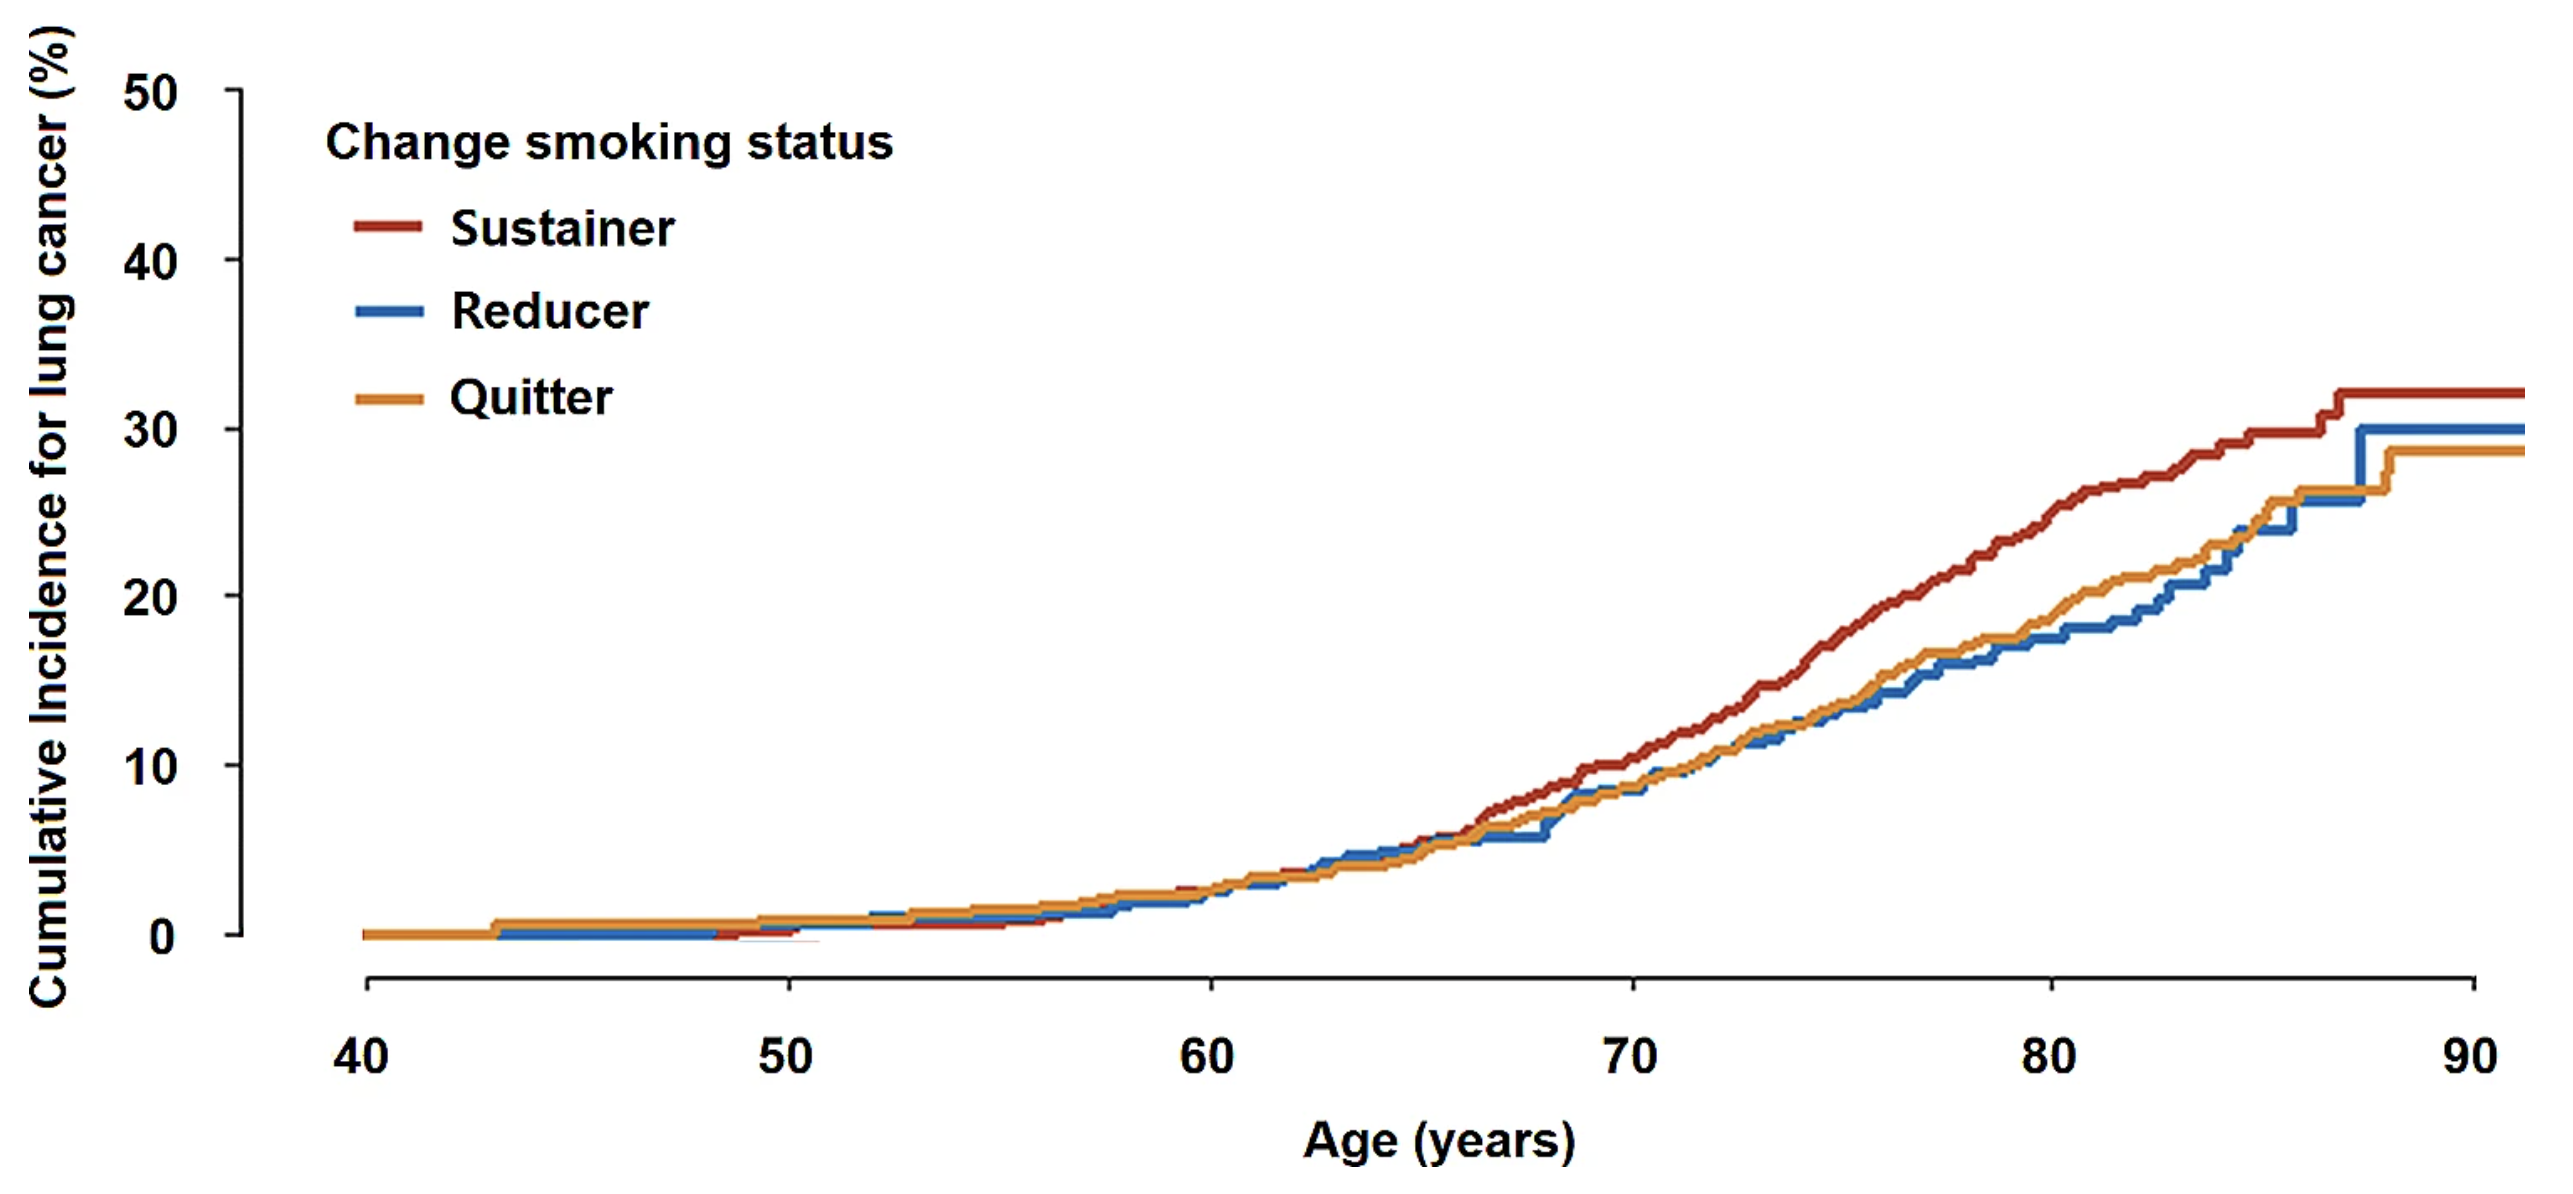
\includegraphics[width=1.00\textwidth]{../assets/05-prognosis/smoking-clinical-outcomes.png}

    \small\textit{Impact of smoking reduction on lung cancer risk in patients with COPD. 
    \cite{shin2024impact}}
\end{center}
\vspace{1em}

% Summary emphasizing how integrating these indicators helps refine prognosis and treatment.
Understanding these prognostic indicators allows healthcare providers to make informed decisions 
regarding treatment intensity, follow-up strategies, and patient counseling. As precision medicine 
advances, integrating clinical, molecular, and lifestyle data will continue to refine prognostic 
models for lung cancer patients.
